Cars are modelled as individual agents, the \code{Car} class inherits MASON's \code{Steppable} interface which allows Cars to be treated as agents by the simulation's Scheduler and have their \code{step()} method called at every timestep in the simulation. Here we will discuss the \code{step()} method, what it does, and why. First though, we must understand how an agent percieves the world around it.

Modern processors no longer necessitate using CA environments in ABM, allowing continuous systems to simulate emergent behaviour with a greater spatial fidelity. Agents in this model exist in such a continuous 2D space, but this presents challenges. Most trivially, the N-S algorithm must be adapted to work for continuous environments, however this is easily overcome as the design of N-S does not strictly require a discrete coordinate space to function. Adapting the N-S algorithm merely requires an adjustment to cases where the agent must slow down due to another car in front of it. Where discrete N-S slows an agent down so that it comes to occupy the cell immediately behind the cell of the car in front of it, continuous N-S slows the same agent down so that its position is some arbitrary stopping distance behind the car in front of it.

A more difficult problem brought about by the environment is implementing agents that follow the roads, and designing how an agent will process nearby cars into its own perception of the road ahead. The solution to this problem is found by giving agents access to the real, 2D, global space as well as a second \textit{network space} within which they can process their surroundings.

\subsection{Network Space}

Network space is a \textit{one-dimensional} coordinate system defined by an agent's current position along the length of a 1D vector of a road segment, we shall call this current length along a road the \textit{index}. Network space is best understood using an example, with Figure \ref{fig:network_space} for reference:

\vspace{1cm}
\begin{figure}[ht]
    \centering
    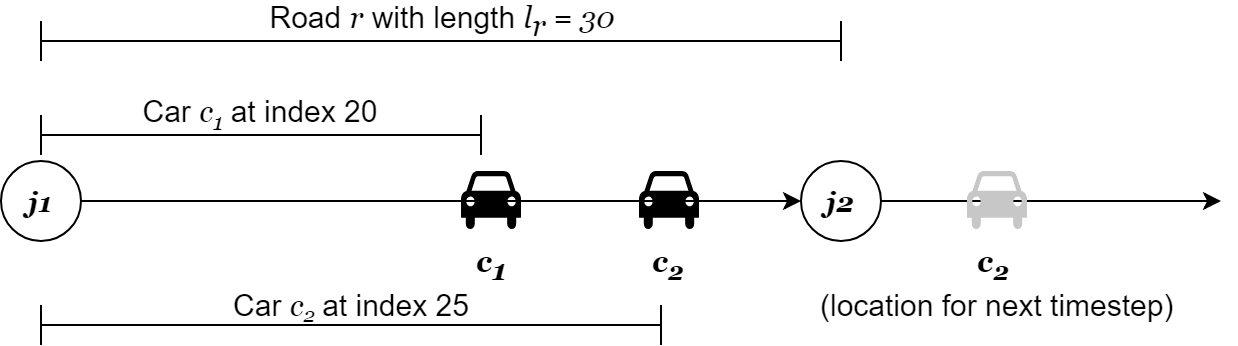
\includegraphics[width=0.8\textwidth]{images/network_space.png}
    \caption{Network Space road traversal}
    \label{fig:network_space}
\end{figure}
\vspace{1cm}
Let $r$ be a road of length $l_r$ = 30 units, directed from a junction $j_1$ towards a junction $j_2$. Suppose a car $c_1$ is positioned 20 units along the road, then the \textit{index} of $c_1$ on $r$ is equal to 20. Suppose the next car ahead of $c_1$, being $c_2$, is 5 units in front, the index of $c_2$ on $r$ is equal to 25. By definition, if the index of a car on road $r$ reaches $l_r$ then that car must have traversed the length of the road and reached the road's destination node, $j_2$.

Here we have been able to reduce a car's two dimensional road behaviour to one dimension. In compliment with the network space, cars still exist in and move through the global 2D space - this facilitates agents that are able to perceive and react not only to the roads but also any other feature in their vicinity. None of the experiments in the scope of this project take advantage of this capability, but potential applications of the feature include allowing cars to interact with pedestrians in the 2D space, and programming cars to react to seeing fire or some other hazard anywhere in the environment. 

As cars move through network space, a transformation is needed to calculate their location in global space. For a car, $c$ at a network space index $i$ on a road $r$ of length $l_r$ from junction $v$ to junction $w$, the global space position of $c$, $p_c$, is given by:

\begin{equation}
    p_c \;=\; v + i\cdot\hat{vw} \;=\; v + i(\frac{\vec{vw}}{l_r})
    \label{eq:vector_global}
\end{equation}

The $x$ and $y$ coordinates of $c$ are found by separating equation \ref{eq:vector_global} into its $x$ and $y$ components:

\begin{equation}
    x_c \;=\; v_x + i(\frac{x_w - x_v}{l_r})
    \label{eq:vector_global}
\end{equation}

\begin{equation}
    y_c \;=\; v_y + i(\frac{y_w - y_v}{l_r})
    \label{eq:vector_global}
\end{equation}

\subsection{Traversing Network Space}
Returning to our earlier example of network space: if $c_2$, which is at index 25, has a velocity greater than 5 in the current timestep then its new index must exceed the length of road $r$, therefore it must travel through the junction $j_2$ and travel onto the next road segment with some residual movement as seen in Figure \ref{fig:network_space}. This next road segment is determined by the evacuation route which $c_2$ had previously calculated to reach its evacuation destination. Hence the general idea of an agent's \code{step()} algorithm falls into place:

\vspace{0.5cm}
\begin{algorithm}[H]
    \SetKwData{Overbreaking}{overbreakingFactor}
    \SetKwFunction{NextCar}{DistanceToNextCar}
    \SetKwFunction{NextEdge}{MoveToNextEdge}
    \SetKwFunction{Location}{CalculateLocation}
    \SetKwFunction{Max}{Max}
    // Adapted N-S Algo:
    
    \uIf{$velocity < speed\_limit$}{
        $velocity \leftarrow velocity + acceleration$\;
    }
    
    \uIf{$\NextCar{car} < velocity$}{
        $velocity \leftarrow \NextCar{car} - bufferBetweenVehicles$\;
    }
    
    \uIf{with probability p}{
        $velocity \leftarrow velocity - overbreakingFactor$\;
    }
    $velocity \leftarrow \Max{0,velocity}$\;
    
    // N-S algo ends
    \BlankLine
    $index \leftarrow index + velocity$\;
    \uIf{$index > roadLength$}{
        $residualMovement \leftarrow index-roadLength$\;
        \NextEdge{residualMovement}\;
    }
    
    \Location{}\;
    
    \caption{A naïve car step method}
    \label{alg:naive_step}
\end{algorithm}
\vspace{0.5cm}


In Algorithm \ref{alg:naive_step}, the \code{MoveToNextEdge()} psuedocode method would perform the necessary steps to load an agent onto a new road segment and it would check if the residual movement is great enough that the agent would traverse the entirety of the new road in a single step. In such a case, \code{MoveToNextEdge()} will be called again with whatever remainder of the step movement is to carry forward to the \textit{next} road segment. This will occur of road segments are exceptionally small and an agent can traverse multiple edges in one time step. As agents are called in random sequence, if an unexpected car joins the agent's route at an upcoming junction, it will be perceived by the agent during their step method. 

It is imperative that \code{DistanceToNextCar()} finds the distance to the next car on the route, regardless of how many roads away such a car is. A first implementation of the agent's naïve step only searched for a next car on the current road segment, however this broke down if no neighbour was found but a neighbour existed at a very low index on the \textit{next} road; the agent would move to the next road and either completely skip over the car which was supposed to be in front of it, or if it tried to leave a buffer between it and the newly found neighbour, it would have to reverse the process of moving edge and replace itself on the old edge. To avoid excessive loading and unloading of agents onto roads, the agent looks ahead in its route for the next neighbour. In practicality, the source code is far more complex than Algorithm \ref{alg:naive_step} and the proper Java method \code{Car.calculateDistanceToNeighbour()} which realises the functionality of this psuedocode method and uses a perception distance outside of which an agent cannot see, hence the search for a next neighbour is bounded.


\subsection{Adding Complexity}

The Naïve Step algorithm works for all simple driving models, however the algorithm fails when complexity is introduced to the car-agent's decision making process, such as when agent greed and road throttling are introduced.

Maths for interpolation n tings
    
Initial loading onto network error